\documentclass[a4paper]{article}
\usepackage{amsmath}
\usepackage[english]{babel}
\usepackage{float}
\usepackage{graphicx}
\usepackage{hyperref}
\usepackage[utf8]{inputenc}
\usepackage{listings}
\usepackage{xcolor}

% Sensible defaults for lstlistings
\lstset{
  basicstyle=\footnotesize\ttfamily,
  belowcaptionskip=1\baselineskip,
  breaklines=true,
  commentstyle=\bfseries\color{purple!40!black}
  frame=L,
  identifierstyle=\color{blue},
  keywordstyle=\bfseries\color{green!40!black},
  language=python,
  showstringspaces=false,
  stringstyle=\color{orange},
  xleftmargin=\parindent,
}

\title{\vspace{-5cm} Assignment 1}
\author{Silvan Robert Adrian}

\begin{document}
\maketitle

% Usually unnecessary, but this simplifies grading for us TAs
\tableofcontents

\section{Make Your Own}

% Enumerations are more lightweight than subsections
\begin{enumerate}
  \item I would take the average Grade $\epsilon$\{A,B,C,D,E,F\}, ECTS in Math $\epsilon$\{N\}, Study Programm (if Computer Science Student or not) $\epsilon$\{0,1\} as values for X.
  \item Grade from the grading scale, y $\epsilon$\{A,B,C,D,E,F\}
  \item I would use a least square lost function. $ \ell(Y',Y) = \sum_{n=1}^{n}(Y-Y')^{2}$
  \item I would use a validation set, from where an unbiased estimator of the expected lost can be calculated using the loss function. This would be an indicator of the performance. 
  \item Possible Issues: that the algorithm does not generalize well (some years tend to have more students of a certain profile, grading system is different etc.), collected information does not at all correlate with the final grade of the student and so on.

\end{enumerate}

\section{Illustration of Markov's and Chebychev's Inequalities}

\begin{figure}[H]
  \centering
  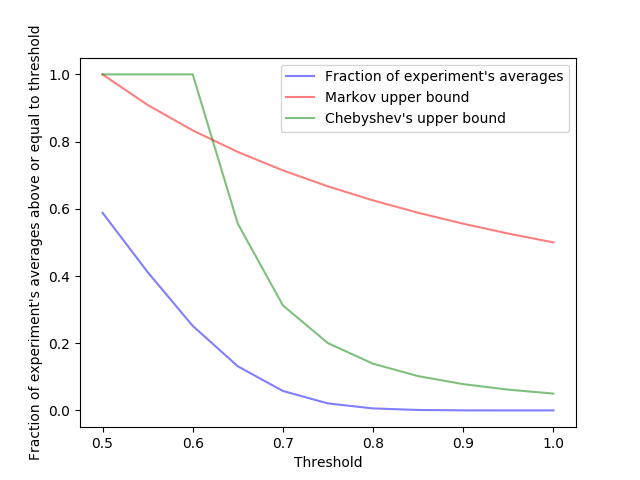
\includegraphics[width=\textwidth]{code/markov_chebychev.png}
  \caption{Representation of fraction of experiments above or equal to the threshold. In blue there is the empirical fraction, while in green and red its upper bound was computed using Chebyshev's and Markov's inequalities respectively. }
  \label{fig:plot_bounds}
\end{figure}
2. In \ref{fig:plot_bounds} blue we can observe the empirical frequency of binary 0,1 experiments which mean is bigger or equal than a certain threshold.  \\\\
3. There are only certain values that the mean can take, which in this case only includes steps of 0.05 (until 1).
	So the probability of having a number bigger or equal than 0.51 is the same than 0.55.\\\\
4. Markov bound can be observed in red in  \ref{fig:plot_bounds}. In order to calculate the Markov bound, the mean of the distribution of outcomes on 20 coin tosses was assumed to be equal to the mean of a single Bernoulli trial with the value 0.5. \\\\
5. In green Chebyshev's bound might be seen in \ref{fig:plot_bounds}. Variance was calculated by central limit theorem ($0.5*0.5*20^{-1}$). The bound was limited to probability values less or equal than 1.\\\\
6. The frequency of experiments averages over or equal a certain $\alpha$ decreases exponentially (blue line), nevertheless Markov bound decreases in a much slow rate (it is a less robust upper bound since is far from the estimated expectation). Chebyshev's for low thresholds do not perform well, it is highly loose. For higher thresholds, it becomes a better bound that Markov, thanks to the fact that it takes into account the amount of samples used ($1^{6}$).\\\\
7. The probability of observing the mean of an experiment over or equal 0.95 is the same than getting 19 out of 20 coins flipping on the same side. This can be calculated as a binomial distribution(p=0.5,n=20).\\
$ P(x \geq 19) = P(X=19) + P(X=20) = 20*0.5^{19}*0.5 + 0.5^{20}= 1.907349e-05 + 9.536743e-07 = 2.002716e-05$\\\\
For being equal or bigger than 1 is the same than equal to one, which can be modeld as a binomial(p=0.5,n=20) of getting 20 out of 20 coins flipping to the same side. \\
$ P(X=20) = 0.5^{20} = 9.536743e-07$

\section{Tightness of Markov's Inequality}
Given the equality:
$\frac{E(x)}{\epsilon} = P(x\geq\epsilon)$ \\\\
For a random variable $X\in\{0,\epsilon\}$ \\\\
$\frac{(0*P(0) + \epsilon*P(\epsilon))}{\epsilon} = P(\epsilon)$ 
As there are only two numbers $P(x\geq\epsilon) = P(\epsilon) $ \\\\
$\frac{\epsilon*P(\epsilon))}{\epsilon} = P(\epsilon)$ ; 
$P(\epsilon)= P(\epsilon)$

\section{Digits Classification with Nearest Neighbours}

\begin{figure}[H]
	\centering
	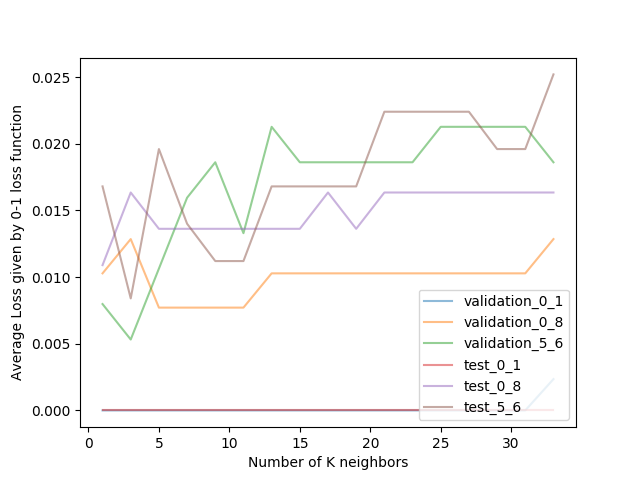
\includegraphics[width=\textwidth]{code/loss_knn_plot}
	\caption{Representation of the loss of K-nn classifier for different Ks. In the legend the different classifications can be seen. The prefix Val makes reference to the usage of the validation dataset (Last 20\% of train dataset) while test uses the complete test dataset for calculating the loss. Pease note validation 0-1 and test 0-1 overlap.}
	\label{fig:plot_error}
\end{figure}

\subsection{How well does the validation error match the test error?}

The figures show a similar pattern. Generally with a higher error in the test than in the validation dataset.\\

\subsection{How closely does the best value of K according to the validation error
match the best value of K according to the test error?}
They are really close, 5-6 and 0-1 totally agree, while 0-8 even though shows a really similar trend do not match their maximum minimum.

\subsection{How the validation and test errors behave as a function of K?} 
The error is correlated with the value of K. This correlation tends to increase the error with higher Ks, but there are some intermediate regions of low error.


\subsection{Does the best value of K depend on the difficulty of the task and how?}
(It is easier to tell apart “0” and “1” than “5” and “6”; the difficulty
of separating “0” and “8” should be somewhere in between.)

0-1 is the easiest classification and is seem since the best value of K is almost any value for both validation and test. 0-8, seems to prefer low and intermediate k values, while the most difficult task requires low values of k (particularly 3). This can be due to the fact that there are much more differences between the numbers and if further away correlations are chosen many miss labels will be taken on the way.


\section{Nearest Neighbours for Multiclass Classification}
 K Nearest Neighbors (K-NN) for Multiclass Classification with Y = \{1, -1\} \\
1: Input: Training labeled points {(x1 ,y1 ),...,(xn ,yn )} and a point x that has to be classified. \\
2: Calculate the distances dist = d(xi ,x). \\
3: Sort dist in ascending order. \\
4: For each position calculate the cummulative mode of the labels. \\
5: The mode of a certain position (k) presents the classification given by K neighbors.



\section{Linear Regression}

\begin{enumerate}
  \item See \texttt{code.zip}
  \item W1 or line slope:  9.4893 ;  b or intercept:  -10.4269 
  \item You find the plot here: \ref{fig:plot_regression}.
    \begin{figure}[H]
      \centering
      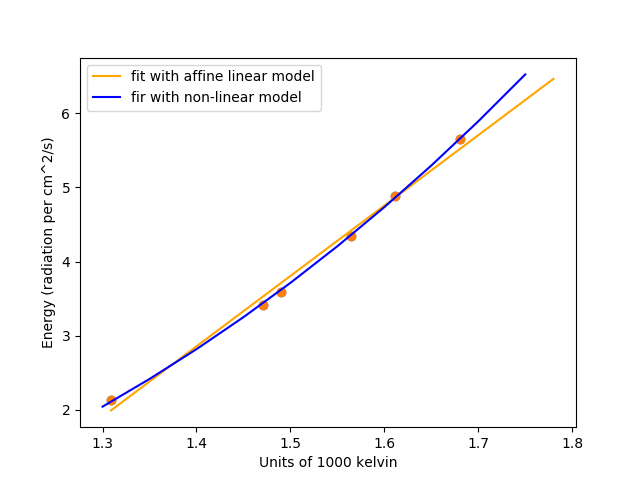
\includegraphics[width=\textwidth]{code/linear_regression}
      \caption{Linear regression of thousands Kelvin degrees vs energy. The scatter dots represent the data points. Two different linear models were adjusting by using Least Squares. In orange a simple affine linear model, while in blue, the data was transformed using $X^{3}$ before using least squares.}
      \label{fig:plot_regression}
    \end{figure}
  \item Error: 0.012434221615054074, variance= 1.2689295555555555 ; Quotient: 0.009798984948073176. \\ The quotient is much lower than 1. This means that the spread of data across the regression line is lower than the spread of data across its mean. If the regression line were constant and at the mean, this coefficient would be one. This would mean that there is no linear correlation between both variables. This coefficient is not expected to be bigger than 1, in non-linear models the best solution will be at least the mean and if the least squares is calculated from a predictor that corresponds to the mean, both the variance and loss are equal.
  
 \item Independent b or intercept:-1.0663,  W1 or line slope: 1.4163. The error: 0.0005. The plot can be seen in \ref{fig:plot_regression}.
\end{enumerate}

\end{document}